% This version of CVPR template is provided by Ming-Ming Cheng.
% Please leave an issue if you found a bug:
% https://github.com/MCG-NKU/CVPR_Template.

\documentclass[final]{cvpr}

\usepackage{times}
\usepackage{epsfig}
\usepackage{graphicx}
\usepackage{amsmath}
\usepackage{amssymb}
\usepackage[french]{babel}
\usepackage[utf8]{inputenc}
\usepackage{subcaption}
\captionsetup{compatibility=false}
% Include other packages here, before hyperref.

% If you comment hyperref and then uncomment it, you should delete
% egpaper.aux before re-running latex.  (Or just hit 'q' on the first latex
% run, let it finish, and you should be clear).
\usepackage[pagebackref=true,breaklinks=true,colorlinks,bookmarks=false]{hyperref}


\def\cvprPaperID{****} % *** Enter the CVPR Paper ID here
\def\confYear{CVPR 2021}
%\setcounter{page}{4321} % For final version only


\begin{document}

%%%%%%%%% TITLE
\title{Sign Language Translation from Video to Text}

\author{Marius \textsc{Schmidt-Mengin}\\
	École des Ponts ParisTech\\
	{\tt\small marius.schmidt.mengin@gmail.com}
% For a paper whose authors are all at the same institution,
% omit the following lines up until the closing ``}''.
% Additional authors and addresses can be added with ``\and'',
% just like the second author.
% To save space, use either the email address or home page, not both
\and
Clément \textsc{Grisi}\\
École des Ponts ParisTech\\
{\tt\small grisi.clement@gmail.com}
}

\maketitle


%%%%%%%%% ABSTRACT
\begin{abstract}
   abstract
   \vspace{5cm}
\end{abstract}

%%%%%%%%% BODY TEXT
\section{Introduction}

%-------------------------------------------------------------------------
\subsection{Sign Language Translation}

explain Sign2Text, Gloss2Text, Sign2Gloss2Text, Sign2(Gloss+Text)

explain dataset


\subsection{Sign Language Transformers}

Here we briefly present Sign Language Transformers \cite{neccam}. We adopt the same notations as in the paper. First, embeddings are extracted from each video frame using a 2D CNN
$$f_{t}= \text{SpatialEmbedding} \left(I_{t}\right) \forall t\in[1, T]$$
This sequence of embeddings is then passed through a Transformer encoder, producing a sequence of encoded spatial embeddings that are then mapped to glosses with a linear layer for sign language recognition. As the number of spatial embeddings may be different from the number of gloss tokens, the Connectionist Temporal Classification (CTC) loss is used. The output of the encoder (before the gloss prediction layer) is passed to the transformer decoder. The decoder also takes as input the target sentence, prepended with a Start Of Sequence (SOS) token, and is trained as in a classical autoregressive seq2seq model. Therefore, Sign Language Transformers learn to predict glosses and sentences jointly.


%-------------------------------------------------------------------------
\section{Video Representations}
\subsection{Spatial Embeddings}

In \cite{neccam}, the spatial embeddings are extracted from a pre-trained 2D CNN. Notably, the 2D CNN they use for their experiments is pre-trained on sign language video \cite{hmm}. The authors of \cite{neccam} showed that this is crucial to achieve good performance, as embeddings extrated from an EfficientNet \cite{effnet} pre-trained on ImageNet are substentially worse on the Sign2Gloss task (the reported WER is almost halved).
It is worth noting that this 2D CNN feature extractor is not trained jointly with the Sign Language Transformer.
\subsection{Spatio-Temporal Embeddings}
We investigate replacing the 2D CNN by a 3D CNN. Our goal is to pre-train this 3D CNN to extract good representations of sign language videos for the Sign2Text task. Training it end-to-end with the Sign Language Transformer is difficult because this requires a lot of GPU memory. Indeed, the input videos can have many frames (up to 475 in the PHOENIX-2014T \cite{phoenix} dataset) and cannot easily be split into multiple part since they are paired with a sentence. Although one possibility would be to reduce the framerate, we prefer to experiment with techniques that do not require textual targets. We experiment with several self-supervised pre-training tasks.
\subsection{Self-Supervised Learning of Video Representations}
Recently, there has been a growing interest in self-supervised learning for image, video, audio or text data. Self-supervised learning allows to leverage large quantities of unlabeled data. Multiple approaches have been explored for self-supervised learning from videos. We explore two of them: predicting whether a video is played forward or backward \cite{arrow} and predicting the order of shuffled clips \cite{vcop}. Other approaches include learning from temporaly modified videos \cite{playback-rate, pace, temp-trans}, learning to predict the future \cite{pred-coding} and contrastive learning \cite{bert-video}.
\subsubsection{Learning from the Arrow of Time}
It has been shown \cite{arrow} that learning to predict if a video clip is played forward or backward can be useful to learn good representations of videos. Our intuition tells us that this task may be particularly well adapted for learning high-level representations of sign language videos since it is very hard to solve for humans that do not know sign language.

\subsubsection{Predicting the Order of Shuffled Clips}
The goal of this task is to predict the order of different clips in a video. More specifically, given some video, several (in general, 3) non-overlapping clips are extracted. A random permutation is chosen (in the case of 3 clips, there are 6 possible permutations). Each of them is then passed through the 3D CNN and average-pooled to a feature vector. The feature vectors of all the clips are concatenated and passed through a 2-layer MLP-like neural network, which predicts the permutation of the clips. Intuitively, only high-level features allow to predict the order of non-overlapping clips.
\subsection{Human Keypoint Estimation}
\subsubsection{Modelling the Body Pose}
Sign language being visual, signers rely on multiple complementaty channels to convey information. These can be grouped into two main categories: manual and non-manual features. Manual features mainly correspond to the hand shape and its motion through time. Although these can be considered as the dominant part of the sign morphology, they alone do not encapsulate the full context of the conveyed information. To give clarity, emphasis and additional meaning, signers use non-manual features, such as facial expressions, mouth gesture, mouthings and body pose. This motivates our work to investigate whether explicitly modelling the body pose (hands, face, upper body) could benefit neural sign language translation.
\subsubsection{Whole-body 3D Pose Estimation}
In order to extract 2D and 3D body keypoints, we applied a pre-trained version of DOPE \cite{dope} to each frame in the PHOENIX-2014T dataset (Figure \ref{fig:2d_3d}). We slighltly modified the code provided by the authors in order to extract for each frame the 2D and 3D whole-body keypoints (face, hands, body) as well as various pooling embeddings (average pooling, max pooling, argmax pooling). The obtained human keypoints were normalized by the mean and standard deviation of the corresponding body part and used as additional input to our sign language transformer model, together with the pooling embeddings.

\begin{figure}[h]
	\begin{subfigure}[h]{0.5\linewidth}
		\centering
			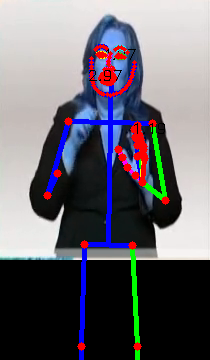
\includegraphics[width=4cm]{fig/toy_DOPE_v1_0_0_2d.png}
	\end{subfigure}\hfill
	\begin{subfigure}[]{0.5\linewidth}
		\centering
		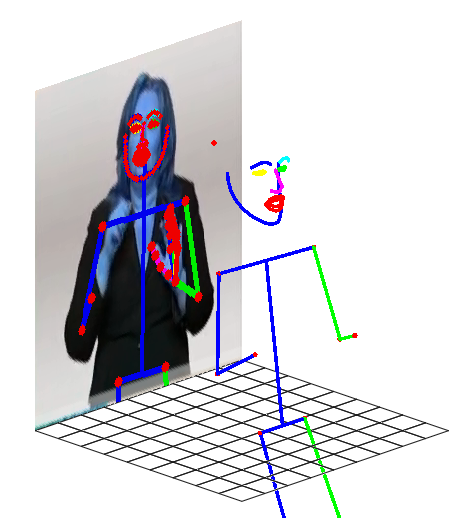
\includegraphics[width=4cm]{fig/toy_DOPE_v1_0_0_3d.png}
	\end{subfigure}
	\caption{2D \& 3D Keypoints on PHOENIX-2014T}
	\label{fig:2d_3d}
\end{figure}

\begin{figure}[h]
		\centering
		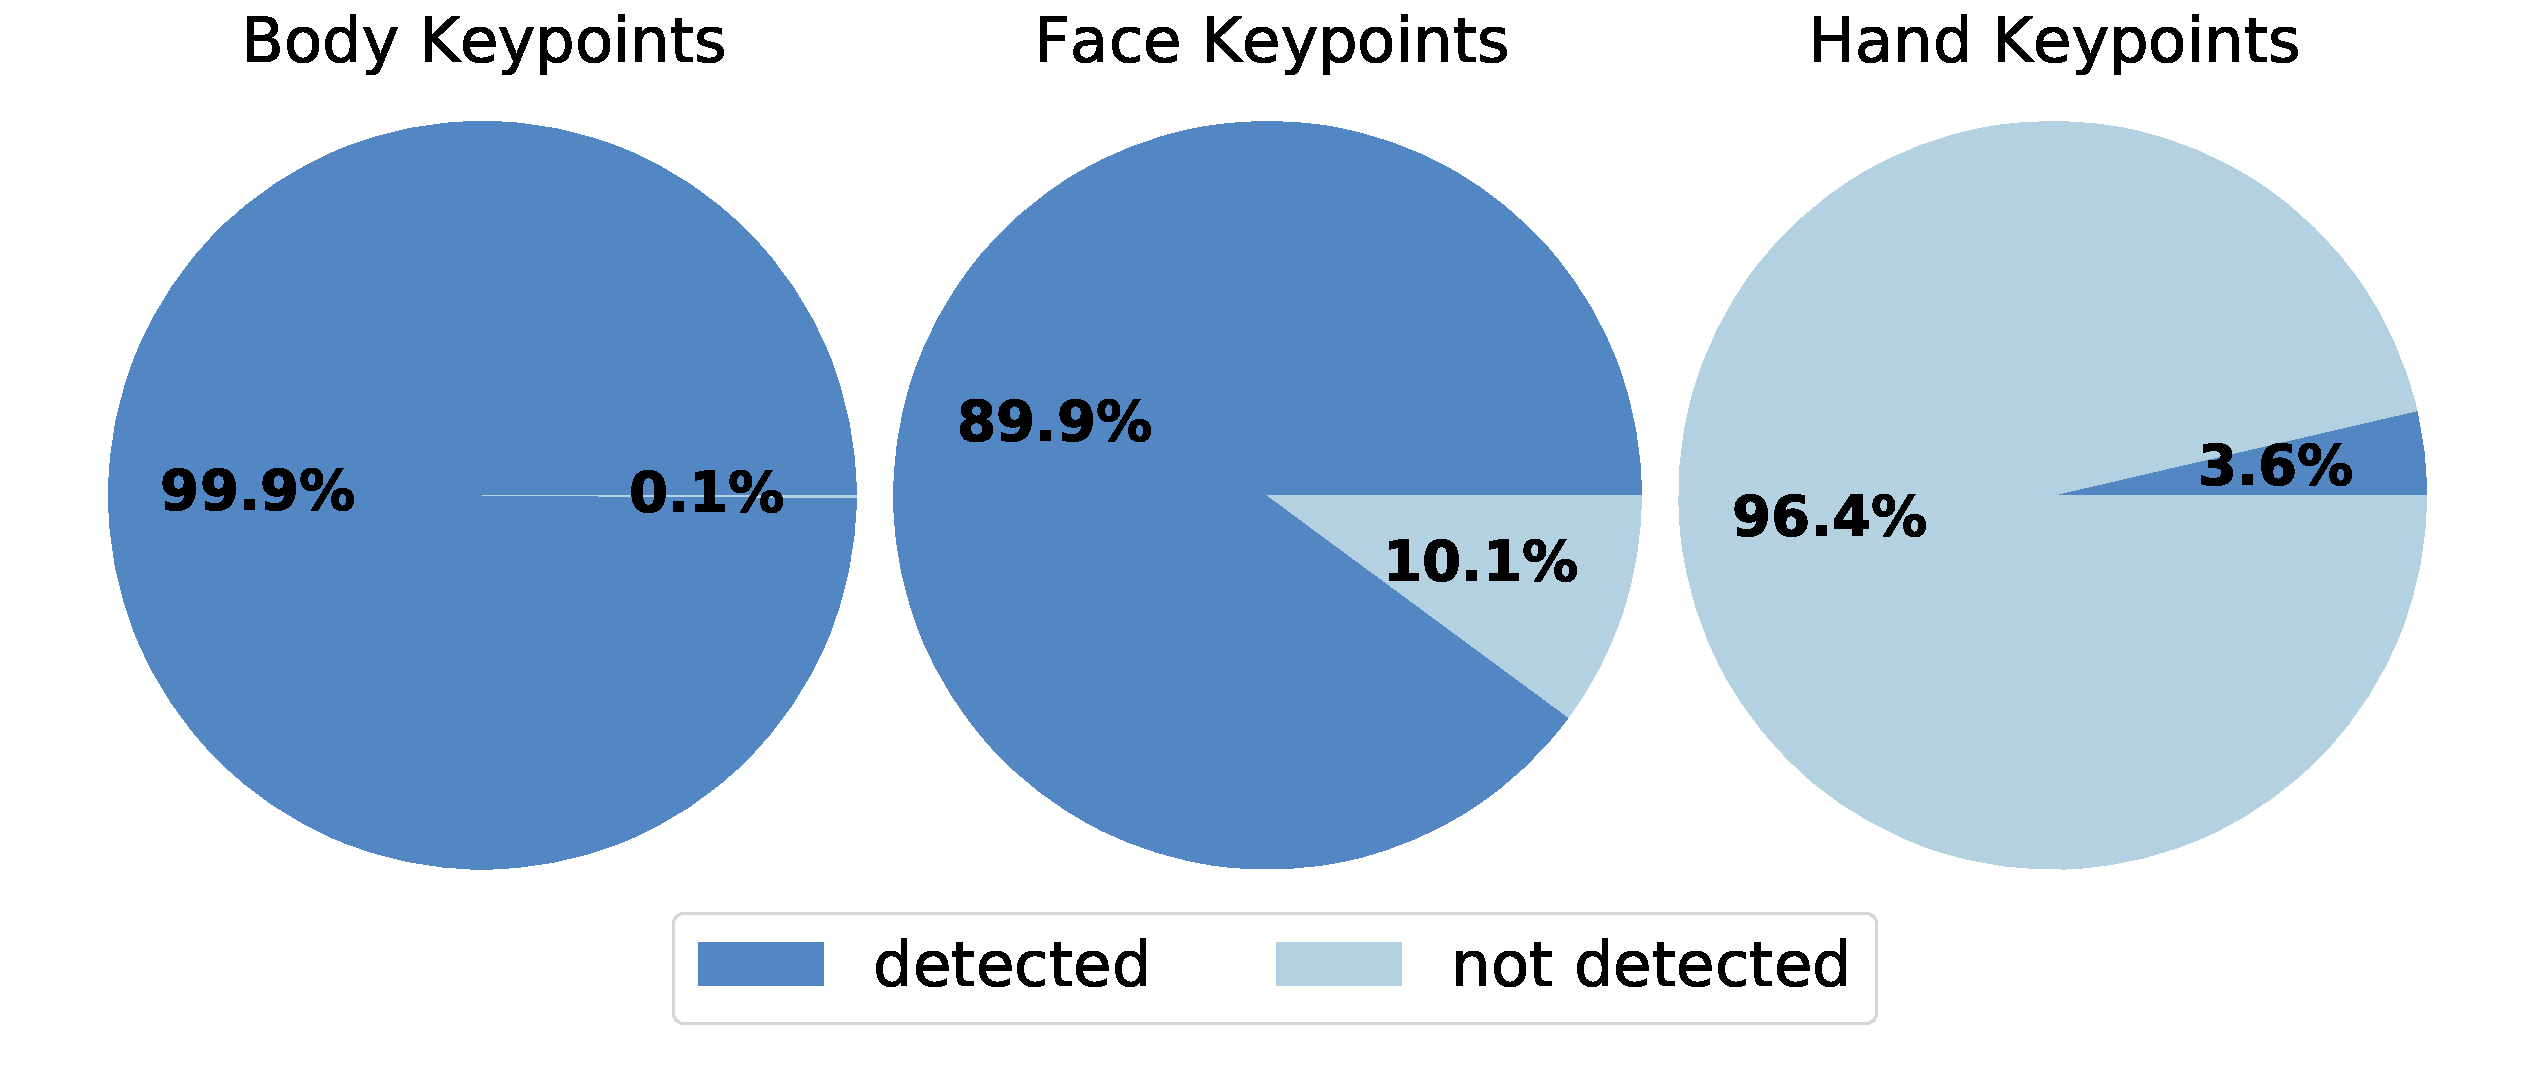
\includegraphics[width=8.7cm]{fig/keypoints.pdf}
	\caption{DOPE Results on  PHOENIX-2014T}
	\label{fig:pie_charts}
\end{figure}


\subsection{DOPE features}

\section{Experiments}
\subsection{Implementation}

To have more flexibility, we re-implement\footnote{\url{https://github.com/marius-sm/sign_language_translation}} Sign Language Transformers \cite{neccam} using Pytorch and HuggingFace transformers \cite{huggingface}. In all our experiments, we use a R(2+1)D \cite{r2plus1} pre-trained on the Kinetics-400 \cite{kinetics} dataset from the Torchvision library as our 3D feature extractor. The last convolutional layer produces 512 channels. Whenever necessary, we average-pool those channels to produce embeddings.

To learn the arrow of time, we use clips of 8 frames and train with a batch size of 32. For clip order prediction, we extract 8 clips from each video with intervals of 8 frames and train with a batch size of 8. We optimize both networks with Adam and a low learning rate of $10^{-5}$ to avoid destroying the Kinetics-400 features.

Once trained, we use these networks to extract the embeddings from all videos. As the dataset videos have significantly more than 8 frames,  extracting the embeddings of a video in a single pass results in a strong train/test discrepancy. To adress this issue, we instead subdivide each video in chunks of 8 frames and extract the embedding of each chunk independently.
\subsection{Qualitative assessments of the embeddings}
After pooling the feature along spatial dimensions, we obtain a sequence of spatial embeddings
$$f_t, t\in[1, ..., \tilde{T}]$$
where $\tilde{T}\leq T$ ($T$ is the number of frames of the input video). For a 2D CNN, $T=\tilde{T}$ whereas R(2+1)D has a temporal stride of $8$, resulting in $\tilde{T} = \lceil T/8 \rceil$.
To assess the quality of our embeddings, we visualize their cosine similarities. Given two videos $v^1$ and $v^2$ and their spatial embeddings sequences $f_t^1, t\in\{1, ..., \tilde{T}^1\}$ and $f_u^2, u\in \{1, ...,  \tilde{T}^2\}$, we compute the matrices $A$ and $B$:
$$A_{tu} = \frac{{f_t^1}^\intercal f_{t'}^1}{\lVert f_t^1 \rVert \lVert f_{t'}^1 \rVert}, \quad\forall t, t' \in\{1, ..., \tilde{T}^1\}$$
$$B_{tu} = \frac{{f_t^1}^\intercal f_u^2}{\lVert f_t^1 \rVert \lVert f_u^2 \rVert}, \quad \forall t \in\{1, ..., \tilde{T}^1\}, u \in\{1, ..., \tilde{T}^2\}$$
That is, we compare the embeddings of a given video with the other embeddings of the same video (matrix $A$) and with the embeddings of another video (matrix $B$). Intuitively, we want 
\begin{itemize}
	\item matrix $A$ to look like a diagonal matrix, where temporaly close frames have similar embeddings, but frames that are far appart have disimilar embeddings, so that there is enough information to recover the translation
	\item matrix $B$ to not have many values close to $1$ as two different videos probably don't translate to related sentences.
\end{itemize}

We first visualize the embeddings of a the 2D CNN pre-trained on sign language data.


{\small
\bibliographystyle{ieee_fullname}
\bibliography{egbib}
}

\end{document}
